% Options for packages loaded elsewhere
\PassOptionsToPackage{unicode}{hyperref}
\PassOptionsToPackage{hyphens}{url}
%
\documentclass[
]{article}
\usepackage{amsmath,amssymb}
\usepackage{iftex}
\ifPDFTeX
  \usepackage[T1]{fontenc}
  \usepackage[utf8]{inputenc}
  \usepackage{textcomp} % provide euro and other symbols
\else % if luatex or xetex
  \usepackage{unicode-math} % this also loads fontspec
  \defaultfontfeatures{Scale=MatchLowercase}
  \defaultfontfeatures[\rmfamily]{Ligatures=TeX,Scale=1}
\fi
\usepackage{lmodern}
\ifPDFTeX\else
  % xetex/luatex font selection
\fi
% Use upquote if available, for straight quotes in verbatim environments
\IfFileExists{upquote.sty}{\usepackage{upquote}}{}
\IfFileExists{microtype.sty}{% use microtype if available
  \usepackage[]{microtype}
  \UseMicrotypeSet[protrusion]{basicmath} % disable protrusion for tt fonts
}{}
\makeatletter
\@ifundefined{KOMAClassName}{% if non-KOMA class
  \IfFileExists{parskip.sty}{%
    \usepackage{parskip}
  }{% else
    \setlength{\parindent}{0pt}
    \setlength{\parskip}{6pt plus 2pt minus 1pt}}
}{% if KOMA class
  \KOMAoptions{parskip=half}}
\makeatother
\usepackage{xcolor}
\usepackage[margin=1in]{geometry}
\usepackage{color}
\usepackage{fancyvrb}
\newcommand{\VerbBar}{|}
\newcommand{\VERB}{\Verb[commandchars=\\\{\}]}
\DefineVerbatimEnvironment{Highlighting}{Verbatim}{commandchars=\\\{\}}
% Add ',fontsize=\small' for more characters per line
\usepackage{framed}
\definecolor{shadecolor}{RGB}{248,248,248}
\newenvironment{Shaded}{\begin{snugshade}}{\end{snugshade}}
\newcommand{\AlertTok}[1]{\textcolor[rgb]{0.94,0.16,0.16}{#1}}
\newcommand{\AnnotationTok}[1]{\textcolor[rgb]{0.56,0.35,0.01}{\textbf{\textit{#1}}}}
\newcommand{\AttributeTok}[1]{\textcolor[rgb]{0.13,0.29,0.53}{#1}}
\newcommand{\BaseNTok}[1]{\textcolor[rgb]{0.00,0.00,0.81}{#1}}
\newcommand{\BuiltInTok}[1]{#1}
\newcommand{\CharTok}[1]{\textcolor[rgb]{0.31,0.60,0.02}{#1}}
\newcommand{\CommentTok}[1]{\textcolor[rgb]{0.56,0.35,0.01}{\textit{#1}}}
\newcommand{\CommentVarTok}[1]{\textcolor[rgb]{0.56,0.35,0.01}{\textbf{\textit{#1}}}}
\newcommand{\ConstantTok}[1]{\textcolor[rgb]{0.56,0.35,0.01}{#1}}
\newcommand{\ControlFlowTok}[1]{\textcolor[rgb]{0.13,0.29,0.53}{\textbf{#1}}}
\newcommand{\DataTypeTok}[1]{\textcolor[rgb]{0.13,0.29,0.53}{#1}}
\newcommand{\DecValTok}[1]{\textcolor[rgb]{0.00,0.00,0.81}{#1}}
\newcommand{\DocumentationTok}[1]{\textcolor[rgb]{0.56,0.35,0.01}{\textbf{\textit{#1}}}}
\newcommand{\ErrorTok}[1]{\textcolor[rgb]{0.64,0.00,0.00}{\textbf{#1}}}
\newcommand{\ExtensionTok}[1]{#1}
\newcommand{\FloatTok}[1]{\textcolor[rgb]{0.00,0.00,0.81}{#1}}
\newcommand{\FunctionTok}[1]{\textcolor[rgb]{0.13,0.29,0.53}{\textbf{#1}}}
\newcommand{\ImportTok}[1]{#1}
\newcommand{\InformationTok}[1]{\textcolor[rgb]{0.56,0.35,0.01}{\textbf{\textit{#1}}}}
\newcommand{\KeywordTok}[1]{\textcolor[rgb]{0.13,0.29,0.53}{\textbf{#1}}}
\newcommand{\NormalTok}[1]{#1}
\newcommand{\OperatorTok}[1]{\textcolor[rgb]{0.81,0.36,0.00}{\textbf{#1}}}
\newcommand{\OtherTok}[1]{\textcolor[rgb]{0.56,0.35,0.01}{#1}}
\newcommand{\PreprocessorTok}[1]{\textcolor[rgb]{0.56,0.35,0.01}{\textit{#1}}}
\newcommand{\RegionMarkerTok}[1]{#1}
\newcommand{\SpecialCharTok}[1]{\textcolor[rgb]{0.81,0.36,0.00}{\textbf{#1}}}
\newcommand{\SpecialStringTok}[1]{\textcolor[rgb]{0.31,0.60,0.02}{#1}}
\newcommand{\StringTok}[1]{\textcolor[rgb]{0.31,0.60,0.02}{#1}}
\newcommand{\VariableTok}[1]{\textcolor[rgb]{0.00,0.00,0.00}{#1}}
\newcommand{\VerbatimStringTok}[1]{\textcolor[rgb]{0.31,0.60,0.02}{#1}}
\newcommand{\WarningTok}[1]{\textcolor[rgb]{0.56,0.35,0.01}{\textbf{\textit{#1}}}}
\usepackage{graphicx}
\makeatletter
\def\maxwidth{\ifdim\Gin@nat@width>\linewidth\linewidth\else\Gin@nat@width\fi}
\def\maxheight{\ifdim\Gin@nat@height>\textheight\textheight\else\Gin@nat@height\fi}
\makeatother
% Scale images if necessary, so that they will not overflow the page
% margins by default, and it is still possible to overwrite the defaults
% using explicit options in \includegraphics[width, height, ...]{}
\setkeys{Gin}{width=\maxwidth,height=\maxheight,keepaspectratio}
% Set default figure placement to htbp
\makeatletter
\def\fps@figure{htbp}
\makeatother
\setlength{\emergencystretch}{3em} % prevent overfull lines
\providecommand{\tightlist}{%
  \setlength{\itemsep}{0pt}\setlength{\parskip}{0pt}}
\setcounter{secnumdepth}{-\maxdimen} % remove section numbering
\ifLuaTeX
  \usepackage{selnolig}  % disable illegal ligatures
\fi
\usepackage{bookmark}
\IfFileExists{xurl.sty}{\usepackage{xurl}}{} % add URL line breaks if available
\urlstyle{same}
\hypersetup{
  pdftitle={Untitled},
  pdfauthor={rachel\_cassway},
  hidelinks,
  pdfcreator={LaTeX via pandoc}}

\title{Untitled}
\author{rachel\_cassway}
\date{2025-04-02}

\begin{document}
\maketitle

\subsubsection{Load and Clean Data}\label{load-and-clean-data}

Getting data into the following format: - Rows = users - Columns =
recipes - Values = ratings (stars)

\begin{Shaded}
\begin{Highlighting}[]
\CommentTok{\# load libraries}
\FunctionTok{library}\NormalTok{(dplyr)}
\end{Highlighting}
\end{Shaded}

\begin{verbatim}
## 
## Attaching package: 'dplyr'
\end{verbatim}

\begin{verbatim}
## The following objects are masked from 'package:stats':
## 
##     filter, lag
\end{verbatim}

\begin{verbatim}
## The following objects are masked from 'package:base':
## 
##     intersect, setdiff, setequal, union
\end{verbatim}

\begin{Shaded}
\begin{Highlighting}[]
\FunctionTok{library}\NormalTok{(tidyr)}
\FunctionTok{library}\NormalTok{(proxy)}
\end{Highlighting}
\end{Shaded}

\begin{verbatim}
## 
## Attaching package: 'proxy'
\end{verbatim}

\begin{verbatim}
## The following objects are masked from 'package:stats':
## 
##     as.dist, dist
\end{verbatim}

\begin{verbatim}
## The following object is masked from 'package:base':
## 
##     as.matrix
\end{verbatim}

\begin{Shaded}
\begin{Highlighting}[]
\FunctionTok{library}\NormalTok{(scales)}

\CommentTok{\# load csv into dataframe}
\NormalTok{df }\OtherTok{\textless{}{-}} \FunctionTok{read.csv}\NormalTok{(}\StringTok{"recipe\_review\_data.csv"}\NormalTok{)}

\CommentTok{\# select collab filtering columns}
\NormalTok{df }\OtherTok{\textless{}{-}}\NormalTok{ df }\SpecialCharTok{\%\textgreater{}\%}
  \FunctionTok{mutate}\NormalTok{(}
    \AttributeTok{user\_id =} \FunctionTok{trimws}\NormalTok{(}\FunctionTok{as.character}\NormalTok{(user\_id)),}
    \AttributeTok{recipe\_code =} \FunctionTok{trimws}\NormalTok{(}\FunctionTok{as.character}\NormalTok{(recipe\_code)),}
    \AttributeTok{stars =} \FunctionTok{as.numeric}\NormalTok{(stars)}
\NormalTok{  )}

\CommentTok{\# clean ratings: take average if user rated the same item multiple times}
\NormalTok{ratings\_cleaned }\OtherTok{\textless{}{-}}\NormalTok{ df }\SpecialCharTok{\%\textgreater{}\%}
  \FunctionTok{filter}\NormalTok{(}\SpecialCharTok{!}\FunctionTok{is.na}\NormalTok{(stars)) }\SpecialCharTok{\%\textgreater{}\%}
  \FunctionTok{group\_by}\NormalTok{(user\_id, recipe\_code) }\SpecialCharTok{\%\textgreater{}\%}
  \FunctionTok{summarise}\NormalTok{(}\AttributeTok{stars =} \FunctionTok{mean}\NormalTok{(stars, }\AttributeTok{na.rm =} \ConstantTok{TRUE}\NormalTok{), }\AttributeTok{.groups =} \StringTok{"drop"}\NormalTok{)}

\CommentTok{\# pivot\_wider, to prep for matrix}
\NormalTok{rating\_wide }\OtherTok{\textless{}{-}}\NormalTok{ ratings\_cleaned }\SpecialCharTok{\%\textgreater{}\%}
  \FunctionTok{pivot\_wider}\NormalTok{(}\AttributeTok{names\_from =}\NormalTok{ recipe\_code, }\AttributeTok{values\_from =}\NormalTok{ stars)}

\CommentTok{\# convert to data.frame before setting rownames}
\NormalTok{rating\_wide }\OtherTok{\textless{}{-}} \FunctionTok{as.data.frame}\NormalTok{(rating\_wide)}

\CommentTok{\# set user\_id as rownames}
\NormalTok{rating\_wide}\SpecialCharTok{$}\NormalTok{user\_id }\OtherTok{\textless{}{-}} \FunctionTok{trimws}\NormalTok{(}\FunctionTok{as.character}\NormalTok{(rating\_wide}\SpecialCharTok{$}\NormalTok{user\_id))}
\FunctionTok{rownames}\NormalTok{(rating\_wide) }\OtherTok{\textless{}{-}}\NormalTok{ rating\_wide}\SpecialCharTok{$}\NormalTok{user\_id}
\NormalTok{rating\_wide }\OtherTok{\textless{}{-}}\NormalTok{ rating\_wide }\SpecialCharTok{\%\textgreater{}\%} \FunctionTok{select}\NormalTok{(}\SpecialCharTok{{-}}\NormalTok{user\_id)}

\CommentTok{\# convert to numeric matrix}
\NormalTok{rating\_wide[] }\OtherTok{\textless{}{-}} \FunctionTok{lapply}\NormalTok{(rating\_wide, }\ControlFlowTok{function}\NormalTok{(x) }\FunctionTok{as.numeric}\NormalTok{(}\FunctionTok{as.character}\NormalTok{(x)))}
\NormalTok{rating\_matrix }\OtherTok{\textless{}{-}} \FunctionTok{as.matrix}\NormalTok{(rating\_wide)}

\CommentTok{\# preview matrix}
\FunctionTok{head}\NormalTok{(rating\_matrix)}
\end{Highlighting}
\end{Shaded}

\begin{verbatim}
##                386 2912 8431 39334 100276 12700 17826 42386 41101 11767 27626
## u_05PZUpOV27Pv   5   NA   NA    NA     NA    NA    NA    NA    NA    NA    NA
## u_09Pspx0F3ZKy  NA    5   NA    NA     NA    NA    NA    NA    NA    NA    NA
## u_0BYS3gNJ4rI0  NA   NA    5    NA     NA    NA    NA    NA    NA    NA    NA
## u_0GfixeKJgmAL  NA   NA   NA     5     NA    NA    NA    NA    NA    NA    NA
## u_0HraB0BMR3qu  NA   NA   NA    NA      0    NA    NA    NA    NA    NA    NA
## u_0S8No1lOgccx  NA   NA   NA    NA     NA     5    NA    NA    NA    NA    NA
##                28058 9735 7708 1196 957 18341 2832 7752 43675 1152 3309 32480
## u_05PZUpOV27Pv    NA   NA   NA   NA  NA    NA   NA   NA    NA   NA   NA    NA
## u_09Pspx0F3ZKy    NA   NA   NA   NA  NA    NA   NA   NA    NA   NA   NA    NA
## u_0BYS3gNJ4rI0    NA   NA   NA   NA  NA    NA   NA   NA    NA   NA   NA    NA
## u_0GfixeKJgmAL    NA   NA   NA   NA  NA    NA   NA   NA    NA   NA   NA    NA
## u_0HraB0BMR3qu    NA   NA   NA   NA  NA    NA   NA   NA    NA   NA   NA    NA
## u_0S8No1lOgccx    NA   NA   NA   NA  NA    NA   NA   NA    NA   NA   NA    NA
##                141947 16579 32264 7539 9010 14299 15805 19731 23222 2872 32248
## u_05PZUpOV27Pv     NA    NA    NA   NA   NA    NA    NA    NA    NA   NA    NA
## u_09Pspx0F3ZKy     NA    NA    NA   NA   NA    NA    NA    NA    NA   NA    NA
## u_0BYS3gNJ4rI0     NA    NA    NA   NA   NA    NA    NA    NA    NA   NA    NA
## u_0GfixeKJgmAL     NA    NA    NA   NA   NA    NA    NA    NA    NA   NA    NA
## u_0HraB0BMR3qu     NA    NA    NA   NA   NA    NA    NA    NA    NA   NA    NA
## u_0S8No1lOgccx     NA    NA    NA   NA   NA    NA    NA    NA    NA   NA    NA
##                39545 41384 11588 12347 36450 38183 7178 12540 39549 16458 1693
## u_05PZUpOV27Pv    NA    NA    NA    NA    NA    NA   NA    NA    NA    NA   NA
## u_09Pspx0F3ZKy    NA    NA    NA    NA    NA    NA   NA    NA    NA    NA   NA
## u_0BYS3gNJ4rI0    NA    NA    NA    NA    NA    NA   NA    NA    NA    NA   NA
## u_0GfixeKJgmAL    NA    NA    NA    NA    NA    NA   NA    NA    NA    NA   NA
## u_0HraB0BMR3qu    NA    NA    NA    NA    NA    NA   NA    NA    NA    NA   NA
## u_0S8No1lOgccx    NA    NA    NA    NA    NA    NA   NA    NA    NA    NA   NA
##                27434 33121 26937 12003 1063 17310 6086 11330 14600 31278 4383
## u_05PZUpOV27Pv    NA    NA    NA    NA   NA    NA   NA    NA    NA    NA   NA
## u_09Pspx0F3ZKy    NA    NA    NA    NA   NA    NA   NA    NA    NA    NA   NA
## u_0BYS3gNJ4rI0    NA    NA    NA    NA   NA    NA   NA    NA    NA    NA   NA
## u_0GfixeKJgmAL    NA    NA    NA    NA   NA    NA   NA    NA    NA    NA   NA
## u_0HraB0BMR3qu    NA    NA    NA    NA   NA    NA   NA    NA    NA    NA   NA
## u_0S8No1lOgccx    NA    NA    NA    NA   NA    NA   NA    NA    NA    NA   NA
##                46655 74724 21444 3290 35948 36217 1081 32535 39581 41095 4444
## u_05PZUpOV27Pv    NA    NA    NA   NA    NA    NA   NA    NA    NA    NA   NA
## u_09Pspx0F3ZKy    NA    NA    NA   NA    NA    NA   NA    NA    NA    NA   NA
## u_0BYS3gNJ4rI0    NA    NA    NA   NA    NA    NA   NA    NA    NA    NA   NA
## u_0GfixeKJgmAL    NA    NA    NA   NA    NA    NA   NA    NA    NA    NA   NA
## u_0HraB0BMR3qu    NA    NA    NA   NA    NA    NA   NA    NA    NA    NA   NA
## u_0S8No1lOgccx    NA    NA    NA   NA    NA    NA   NA    NA    NA    NA   NA
##                6504 82745 9739 10252 12734 20170 33206 3058 191775 42873 18274
## u_05PZUpOV27Pv   NA    NA   NA    NA    NA    NA    NA   NA     NA    NA    NA
## u_09Pspx0F3ZKy   NA    NA   NA    NA    NA    NA    NA   NA     NA    NA    NA
## u_0BYS3gNJ4rI0   NA    NA   NA    NA    NA    NA    NA   NA     NA    NA    NA
## u_0GfixeKJgmAL   NA    NA   NA    NA    NA    NA    NA   NA     NA    NA    NA
## u_0HraB0BMR3qu   NA    NA   NA    NA    NA    NA    NA   NA     NA    NA    NA
## u_0S8No1lOgccx   NA    NA   NA    NA    NA    NA    NA   NA     NA    NA    NA
##                33457 27696 42083 12259 10248 1821 24886 8015 1324 38550 33743
## u_05PZUpOV27Pv    NA    NA    NA    NA    NA   NA    NA   NA   NA    NA    NA
## u_09Pspx0F3ZKy    NA    NA    NA    NA    NA   NA    NA   NA   NA    NA    NA
## u_0BYS3gNJ4rI0    NA    NA    NA    NA    NA   NA    NA   NA   NA    NA    NA
## u_0GfixeKJgmAL    NA    NA    NA    NA    NA   NA    NA   NA   NA    NA    NA
## u_0HraB0BMR3qu    NA    NA    NA    NA    NA   NA    NA   NA   NA    NA    NA
## u_0S8No1lOgccx    NA    NA    NA    NA    NA   NA    NA   NA   NA    NA    NA
##                27675 35766 414 3143 18345 34347 3683 45495 19201 8202 17022
## u_05PZUpOV27Pv    NA    NA  NA   NA    NA    NA   NA    NA    NA   NA    NA
## u_09Pspx0F3ZKy    NA    NA  NA   NA    NA    NA   NA    NA    NA   NA    NA
## u_0BYS3gNJ4rI0    NA    NA  NA   NA    NA    NA   NA    NA    NA   NA    NA
## u_0GfixeKJgmAL    NA    NA  NA   NA    NA    NA   NA    NA    NA   NA    NA
## u_0HraB0BMR3qu    NA    NA  NA   NA    NA    NA   NA    NA    NA   NA    NA
## u_0S8No1lOgccx    NA    NA  NA   NA    NA    NA   NA    NA    NA   NA    NA
\end{verbatim}

\begin{Shaded}
\begin{Highlighting}[]
\CommentTok{\# make sure each recipe is distinct in lookup table}
\NormalTok{recipe\_lookup }\OtherTok{\textless{}{-}}\NormalTok{ df }\SpecialCharTok{\%\textgreater{}\%}
  \FunctionTok{select}\NormalTok{(recipe\_code, recipe\_name) }\SpecialCharTok{\%\textgreater{}\%}
  \FunctionTok{distinct}\NormalTok{(recipe\_code, }\AttributeTok{.keep\_all =} \ConstantTok{TRUE}\NormalTok{)  }
\end{Highlighting}
\end{Shaded}

\subsubsection{Some analysis on data to explore popular recipes and
frequent
users}\label{some-analysis-on-data-to-explore-popular-recipes-and-frequent-users}

\begin{Shaded}
\begin{Highlighting}[]
\CommentTok{\# which users have rated the most recipes}
\NormalTok{user\_rating\_counts }\OtherTok{\textless{}{-}} \FunctionTok{rowSums}\NormalTok{(}\SpecialCharTok{!}\FunctionTok{is.na}\NormalTok{(rating\_matrix))}
\NormalTok{top\_users }\OtherTok{\textless{}{-}} \FunctionTok{sort}\NormalTok{(user\_rating\_counts, }\AttributeTok{decreasing =} \ConstantTok{TRUE}\NormalTok{)}

\FunctionTok{head}\NormalTok{(top\_users)}
\end{Highlighting}
\end{Shaded}

\begin{verbatim}
## u_1oKVZzipo1u8lcqQzDUcw4UBn9e u_1oKVZdmUbQTYMVdbXOpVfRQuHm9 
##                            25                            23 
## u_1oKVZmYPulmUFbvGiBA8U3uRR6D u_1oKVZoIOMWJ2j7TA7py2BIbf1mm 
##                            23                            23 
## u_1oKVeN9YNf07RT0P9R63Yu80P5A u_1oKVZxAOR5BEzyF4H6ENc7jwfUW 
##                            23                            22
\end{verbatim}

\begin{Shaded}
\begin{Highlighting}[]
\FunctionTok{length}\NormalTok{(user\_rating\_counts[user\_rating\_counts }\SpecialCharTok{\textgreater{}=} \DecValTok{10}\NormalTok{])}
\end{Highlighting}
\end{Shaded}

\begin{verbatim}
## [1] 52
\end{verbatim}

\begin{Shaded}
\begin{Highlighting}[]
\CommentTok{\# which recipe has the most ratings}
\NormalTok{recipe\_popularity }\OtherTok{\textless{}{-}}\NormalTok{ df }\SpecialCharTok{\%\textgreater{}\%}
  \FunctionTok{filter}\NormalTok{(}\SpecialCharTok{!}\FunctionTok{is.na}\NormalTok{(stars)) }\SpecialCharTok{\%\textgreater{}\%}
  \FunctionTok{count}\NormalTok{(recipe\_code, recipe\_name, }\AttributeTok{sort =} \ConstantTok{TRUE}\NormalTok{)}

\FunctionTok{head}\NormalTok{(recipe\_popularity)}
\end{Highlighting}
\end{Shaded}

\begin{verbatim}
##   recipe_code             recipe_name   n
## 1        2832       Cheeseburger Soup 725
## 2       14299      Creamy White Chili 654
## 3        3309  Best Ever Banana Bread 509
## 4       42083   Enchilada Casser-Ole! 421
## 5       32480    Basic Homemade Bread 397
## 6       21444 Favorite Chicken Potpie 395
\end{verbatim}

\begin{Shaded}
\begin{Highlighting}[]
\CommentTok{\# users who rated most recipes, with highest user reputation}
\NormalTok{top\_reviewers }\OtherTok{\textless{}{-}}\NormalTok{ df }\SpecialCharTok{\%\textgreater{}\%}
  \FunctionTok{filter}\NormalTok{(}\SpecialCharTok{!}\FunctionTok{is.na}\NormalTok{(stars)) }\SpecialCharTok{\%\textgreater{}\%}
  \FunctionTok{group\_by}\NormalTok{(user\_id, user\_name) }\SpecialCharTok{\%\textgreater{}\%}
  \FunctionTok{summarise}\NormalTok{(}
    \AttributeTok{num\_reviews =} \FunctionTok{n}\NormalTok{(),}
    \AttributeTok{avg\_rating =} \FunctionTok{mean}\NormalTok{(stars),}
    \AttributeTok{user\_reputation =} \FunctionTok{max}\NormalTok{(user\_reputation),}
    \AttributeTok{.groups =} \StringTok{"drop"} 
\NormalTok{  ) }\SpecialCharTok{\%\textgreater{}\%}
  \FunctionTok{arrange}\NormalTok{(}\FunctionTok{desc}\NormalTok{(num\_reviews))}
\end{Highlighting}
\end{Shaded}

\subsubsection{user-user collaborative filtering
function}\label{user-user-collaborative-filtering-function}

\begin{Shaded}
\begin{Highlighting}[]
\NormalTok{user\_user\_cf }\OtherTok{\textless{}{-}} \ControlFlowTok{function}\NormalTok{(df, user, }\AttributeTok{sim\_metric =} \StringTok{"Cosine"}\NormalTok{, }\AttributeTok{k =} \DecValTok{2}\NormalTok{, }
                         \AttributeTok{recipe\_lookup\_df =} \ConstantTok{NULL}\NormalTok{) \{}
  
  \CommentTok{\# if user not in data, return not found message}
  \ControlFlowTok{if}\NormalTok{ (}\SpecialCharTok{!}\NormalTok{(user }\SpecialCharTok{\%in\%} \FunctionTok{rownames}\NormalTok{(df))) \{}
    \FunctionTok{message}\NormalTok{(}\StringTok{"Error: User not found in dataset."}\NormalTok{)}
    \FunctionTok{return}\NormalTok{(}\ConstantTok{NULL}\NormalTok{)}
\NormalTok{  \}}

  \CommentTok{\# if the user has no missing values, return message}
  \ControlFlowTok{if}\NormalTok{ (}\FunctionTok{all}\NormalTok{(}\SpecialCharTok{!}\FunctionTok{is.na}\NormalTok{(df[user, ]))) \{}
    \FunctionTok{message}\NormalTok{(}\StringTok{"User has no missing ratings to predict."}\NormalTok{)}
    \FunctionTok{return}\NormalTok{(}\ConstantTok{NULL}\NormalTok{)}
\NormalTok{  \}}

  \CommentTok{\# if similarity metric not Cosine or L2, return message}
  \ControlFlowTok{if}\NormalTok{ (}\SpecialCharTok{!}\NormalTok{(sim\_metric }\SpecialCharTok{\%in\%} \FunctionTok{c}\NormalTok{(}\StringTok{"Cosine"}\NormalTok{, }\StringTok{"L2"}\NormalTok{))) \{}
    \FunctionTok{message}\NormalTok{(}\StringTok{"Unsupported similarity metric. Use \textquotesingle{}Cosine\textquotesingle{} or \textquotesingle{}L2\textquotesingle{}."}\NormalTok{)}
    \FunctionTok{return}\NormalTok{(}\ConstantTok{NULL}\NormalTok{)}
\NormalTok{  \}}

  \CommentTok{\# 1. center data by row means}
\NormalTok{  user\_means }\OtherTok{\textless{}{-}} \FunctionTok{rowMeans}\NormalTok{(df, }\AttributeTok{na.rm =} \ConstantTok{TRUE}\NormalTok{)}
\NormalTok{  centered\_data }\OtherTok{\textless{}{-}} \FunctionTok{sweep}\NormalTok{(df, }\DecValTok{1}\NormalTok{, user\_means, }\AttributeTok{FUN =} \StringTok{"{-}"}\NormalTok{)}
  \CommentTok{\# fill NaN values with 0 for user{-}user only}
\NormalTok{  centered\_data[}\FunctionTok{is.na}\NormalTok{(centered\_data)] }\OtherTok{\textless{}{-}} \DecValTok{0}  

  \CommentTok{\# 2. get target user vector}
\NormalTok{  user\_vector }\OtherTok{\textless{}{-}} \FunctionTok{as.matrix}\NormalTok{(centered\_data[user, , }\AttributeTok{drop =} \ConstantTok{FALSE}\NormalTok{])}

  \CommentTok{\# 3. compute similarity}
  \ControlFlowTok{if}\NormalTok{ (sim\_metric }\SpecialCharTok{==} \StringTok{"Cosine"}\NormalTok{) \{}
\NormalTok{    sim\_vec }\OtherTok{\textless{}{-}}\NormalTok{ proxy}\SpecialCharTok{::}\FunctionTok{simil}\NormalTok{(user\_vector, centered\_data, }\AttributeTok{method =} \StringTok{"cosine"}\NormalTok{)}
\NormalTok{    similarity\_scores }\OtherTok{\textless{}{-}} \FunctionTok{as.vector}\NormalTok{(sim\_vec)}
\NormalTok{  \} }\ControlFlowTok{else} \ControlFlowTok{if}\NormalTok{ (sim\_metric }\SpecialCharTok{==} \StringTok{"L2"}\NormalTok{) \{}
\NormalTok{    diff }\OtherTok{\textless{}{-}}\NormalTok{ centered\_data }\SpecialCharTok{{-}} \FunctionTok{matrix}\NormalTok{(}\FunctionTok{rep}\NormalTok{(user\_vector, }\FunctionTok{nrow}\NormalTok{(centered\_data)), }
                                   \AttributeTok{nrow =} \FunctionTok{nrow}\NormalTok{(centered\_data), }\AttributeTok{byrow =} \ConstantTok{TRUE}\NormalTok{)}
\NormalTok{    similarity\_scores }\OtherTok{\textless{}{-}} \SpecialCharTok{{-}}\FunctionTok{sqrt}\NormalTok{(}\FunctionTok{rowSums}\NormalTok{(diff}\SpecialCharTok{\^{}}\DecValTok{2}\NormalTok{))}
\NormalTok{  \}}

  \CommentTok{\# 4. normalize similarity}
\NormalTok{  similarity\_scores }\OtherTok{\textless{}{-}} \FunctionTok{rescale}\NormalTok{(similarity\_scores, }\AttributeTok{to =} \FunctionTok{c}\NormalTok{(}\DecValTok{0}\NormalTok{, }\DecValTok{1}\NormalTok{))}
\NormalTok{  sim\_df }\OtherTok{\textless{}{-}} \FunctionTok{data.frame}\NormalTok{(}\AttributeTok{User =} \FunctionTok{rownames}\NormalTok{(df), }\AttributeTok{Similarity =}\NormalTok{ similarity\_scores)}
\NormalTok{  sim\_df }\OtherTok{\textless{}{-}}\NormalTok{ sim\_df }\SpecialCharTok{\%\textgreater{}\%} \FunctionTok{filter}\NormalTok{(User }\SpecialCharTok{!=}\NormalTok{ user)}

  \CommentTok{\# 5. select top k similar users}
\NormalTok{  top\_k\_users }\OtherTok{\textless{}{-}}\NormalTok{ sim\_df }\SpecialCharTok{\%\textgreater{}\%}
  \FunctionTok{arrange}\NormalTok{(}\FunctionTok{desc}\NormalTok{(Similarity)) }\SpecialCharTok{\%\textgreater{}\%}
  \FunctionTok{slice\_head}\NormalTok{(}\AttributeTok{n =} \FunctionTok{min}\NormalTok{(k, }\FunctionTok{nrow}\NormalTok{(sim\_df)))}


  \CommentTok{\# 6. prepare ratings for predictions}
\NormalTok{  k\_ratings }\OtherTok{\textless{}{-}}\NormalTok{ df[top\_k\_users}\SpecialCharTok{$}\NormalTok{User, ]}
\NormalTok{  k\_ratings }\OtherTok{\textless{}{-}} \FunctionTok{t}\NormalTok{(}\FunctionTok{apply}\NormalTok{(k\_ratings, }\DecValTok{1}\NormalTok{, }\ControlFlowTok{function}\NormalTok{(row) \{}
\NormalTok{    row[}\FunctionTok{is.na}\NormalTok{(row)] }\OtherTok{\textless{}{-}} \FunctionTok{mean}\NormalTok{(row, }\AttributeTok{na.rm =} \ConstantTok{TRUE}\NormalTok{)}
    \FunctionTok{return}\NormalTok{(row)}
\NormalTok{  \}))}

  \CommentTok{\# 7. weighted prediction}
  \ControlFlowTok{if}\NormalTok{ (}\FunctionTok{sum}\NormalTok{(top\_k\_users}\SpecialCharTok{$}\NormalTok{Similarity) }\SpecialCharTok{==} \DecValTok{0}\NormalTok{) \{}
    \FunctionTok{message}\NormalTok{(}\StringTok{"Warning: All similarities are zero. Returning NULL."}\NormalTok{)}
    \FunctionTok{return}\NormalTok{(}\ConstantTok{NULL}\NormalTok{)}
\NormalTok{  \}}

  \CommentTok{\# calc ratings}
\NormalTok{  weighted }\OtherTok{\textless{}{-}} \FunctionTok{sweep}\NormalTok{(k\_ratings, }\DecValTok{1}\NormalTok{, top\_k\_users}\SpecialCharTok{$}\NormalTok{Similarity, }\AttributeTok{FUN =} \StringTok{"*"}\NormalTok{)}
\NormalTok{  predicted\_ratings }\OtherTok{\textless{}{-}} \FunctionTok{colSums}\NormalTok{(weighted) }\SpecialCharTok{/} \FunctionTok{sum}\NormalTok{(top\_k\_users}\SpecialCharTok{$}\NormalTok{Similarity)}

  \CommentTok{\# return missing predictions only for target user}
\NormalTok{  result }\OtherTok{\textless{}{-}} \FunctionTok{data.frame}\NormalTok{(}\AttributeTok{recipe\_code =} \FunctionTok{colnames}\NormalTok{(df), }\AttributeTok{Predicted\_Rating =}\NormalTok{ predicted\_ratings)}
\NormalTok{  missing\_items }\OtherTok{\textless{}{-}} \FunctionTok{is.na}\NormalTok{(df[user, ])}
\NormalTok{  result }\OtherTok{\textless{}{-}}\NormalTok{ result[missing\_items, ]}
  
  \CommentTok{\# add recipe names if provided in original df}
  \ControlFlowTok{if}\NormalTok{ (}\SpecialCharTok{!}\FunctionTok{is.null}\NormalTok{(recipe\_lookup\_df)) \{}
\NormalTok{    result }\OtherTok{\textless{}{-}}\NormalTok{ result }\SpecialCharTok{\%\textgreater{}\%}
      \FunctionTok{left\_join}\NormalTok{(recipe\_lookup\_df, }\AttributeTok{by =} \StringTok{"recipe\_code"}\NormalTok{) }\SpecialCharTok{\%\textgreater{}\%}
      \FunctionTok{select}\NormalTok{(recipe\_code, recipe\_name, Predicted\_Rating)}
\NormalTok{  \}}

\NormalTok{  result }\OtherTok{\textless{}{-}}\NormalTok{ result }\SpecialCharTok{\%\textgreater{}\%}
    \FunctionTok{arrange}\NormalTok{(}\FunctionTok{desc}\NormalTok{(Predicted\_Rating))}
  
  \FunctionTok{return}\NormalTok{(result)}
\NormalTok{\}}
\end{Highlighting}
\end{Shaded}

\subsubsection{item-item collaborative filtering
function}\label{item-item-collaborative-filtering-function}

\begin{Shaded}
\begin{Highlighting}[]
\NormalTok{item\_item\_cf }\OtherTok{\textless{}{-}} \ControlFlowTok{function}\NormalTok{(df, user, }\AttributeTok{sim\_metric =} \StringTok{"Cosine"}\NormalTok{, }\AttributeTok{k =} \DecValTok{2}\NormalTok{, }
                         \AttributeTok{recipe\_lookup\_df =} \ConstantTok{NULL}\NormalTok{) \{}
  
  \CommentTok{\# if user not in data, return not found message}
  \ControlFlowTok{if}\NormalTok{ (}\SpecialCharTok{!}\NormalTok{(user }\SpecialCharTok{\%in\%} \FunctionTok{rownames}\NormalTok{(df))) \{}
    \FunctionTok{message}\NormalTok{(}\StringTok{"Error: User not found in dataset."}\NormalTok{)}
    \FunctionTok{return}\NormalTok{(}\ConstantTok{NULL}\NormalTok{)}
\NormalTok{  \}}

  \CommentTok{\# if the user has no missing values, return message}
  \ControlFlowTok{if}\NormalTok{ (}\FunctionTok{all}\NormalTok{(}\SpecialCharTok{!}\FunctionTok{is.na}\NormalTok{(df[user, ]))) \{}
    \FunctionTok{message}\NormalTok{(}\StringTok{"User has no missing ratings to predict."}\NormalTok{)}
    \FunctionTok{return}\NormalTok{(}\ConstantTok{NULL}\NormalTok{)}
\NormalTok{  \}}

  \CommentTok{\# if similarity metric not Cosine or L2, return message}
  \ControlFlowTok{if}\NormalTok{ (}\SpecialCharTok{!}\NormalTok{(sim\_metric }\SpecialCharTok{\%in\%} \FunctionTok{c}\NormalTok{(}\StringTok{"Cosine"}\NormalTok{, }\StringTok{"L2"}\NormalTok{))) \{}
    \FunctionTok{message}\NormalTok{(}\StringTok{"Unsupported similarity metric. Use \textquotesingle{}Cosine\textquotesingle{} or \textquotesingle{}L2\textquotesingle{}."}\NormalTok{)}
    \FunctionTok{return}\NormalTok{(}\ConstantTok{NULL}\NormalTok{)}
\NormalTok{  \}}
  
  \CommentTok{\# 1. center by column (item) means}
\NormalTok{  item\_means }\OtherTok{\textless{}{-}} \FunctionTok{colMeans}\NormalTok{(df, }\AttributeTok{na.rm =} \ConstantTok{TRUE}\NormalTok{)}
\NormalTok{  centered\_data }\OtherTok{\textless{}{-}} \FunctionTok{sweep}\NormalTok{(df, }\DecValTok{2}\NormalTok{, item\_means, }\AttributeTok{FUN =} \StringTok{"{-}"}\NormalTok{)}
\NormalTok{  centered\_data[}\FunctionTok{is.na}\NormalTok{(centered\_data)] }\OtherTok{\textless{}{-}} \DecValTok{0}

  \CommentTok{\# 2. transpose for item{-}based similarity (now rows = items)}
\NormalTok{  item\_data }\OtherTok{\textless{}{-}} \FunctionTok{t}\NormalTok{(centered\_data)}

  \CommentTok{\# 3. ratings the user has already made}
\NormalTok{  user\_vector }\OtherTok{\textless{}{-}} \FunctionTok{as.numeric}\NormalTok{(df[user, ])}
  \FunctionTok{names}\NormalTok{(user\_vector) }\OtherTok{\textless{}{-}} \FunctionTok{colnames}\NormalTok{(df)}

\NormalTok{  predictions }\OtherTok{\textless{}{-}} \FunctionTok{numeric}\NormalTok{(}\FunctionTok{ncol}\NormalTok{(df))}
  \FunctionTok{names}\NormalTok{(predictions) }\OtherTok{\textless{}{-}} \FunctionTok{colnames}\NormalTok{(df)}

  \ControlFlowTok{for}\NormalTok{ (item }\ControlFlowTok{in} \FunctionTok{names}\NormalTok{(user\_vector)) \{}
    \CommentTok{\# skip if user already rated it}
    \ControlFlowTok{if}\NormalTok{ (}\SpecialCharTok{!}\FunctionTok{is.na}\NormalTok{(user\_vector[item])) }\ControlFlowTok{next}

    \CommentTok{\# get all items the user has rated}
\NormalTok{    rated\_items }\OtherTok{\textless{}{-}} \FunctionTok{names}\NormalTok{(user\_vector)[}\SpecialCharTok{!}\FunctionTok{is.na}\NormalTok{(user\_vector)]}

    \CommentTok{\# compute similarity between this target item and all items the user rated}
    \ControlFlowTok{if}\NormalTok{ (sim\_metric }\SpecialCharTok{==} \StringTok{"Cosine"}\NormalTok{) \{}
\NormalTok{      sim\_scores }\OtherTok{\textless{}{-}}\NormalTok{ proxy}\SpecialCharTok{::}\FunctionTok{simil}\NormalTok{(}\FunctionTok{as.matrix}\NormalTok{(item\_data[item, , }\AttributeTok{drop =} \ConstantTok{FALSE}\NormalTok{]),}
\NormalTok{                                 item\_data[rated\_items, , }\AttributeTok{drop =} \ConstantTok{FALSE}\NormalTok{],}
                                 \AttributeTok{method =} \StringTok{"cosine"}\NormalTok{)}
\NormalTok{      sim\_scores }\OtherTok{\textless{}{-}} \FunctionTok{as.vector}\NormalTok{(sim\_scores)}
\NormalTok{    \} }\ControlFlowTok{else} \ControlFlowTok{if}\NormalTok{ (sim\_metric }\SpecialCharTok{==} \StringTok{"L2"}\NormalTok{) \{}
\NormalTok{      diff }\OtherTok{\textless{}{-}}\NormalTok{ item\_data[item, ] }\SpecialCharTok{{-}}\NormalTok{ item\_data[rated\_items, ]}
\NormalTok{      sim\_scores }\OtherTok{\textless{}{-}} \SpecialCharTok{{-}}\FunctionTok{sqrt}\NormalTok{(}\FunctionTok{rowSums}\NormalTok{(diff}\SpecialCharTok{\^{}}\DecValTok{2}\NormalTok{))}
\NormalTok{    \}}

    \CommentTok{\# 4. normalize similarity}
\NormalTok{    sim\_scores }\OtherTok{\textless{}{-}} \FunctionTok{rescale}\NormalTok{(sim\_scores, }\AttributeTok{to =} \FunctionTok{c}\NormalTok{(}\DecValTok{0}\NormalTok{, }\DecValTok{1}\NormalTok{))}

    \CommentTok{\# grab the user’s ratings for the similar items}
\NormalTok{    rated\_scores }\OtherTok{\textless{}{-}}\NormalTok{ user\_vector[rated\_items]}

    \CommentTok{\# 5. select top k similar users}
\NormalTok{    top\_k }\OtherTok{\textless{}{-}} \FunctionTok{order}\NormalTok{(sim\_scores, }\AttributeTok{decreasing =} \ConstantTok{TRUE}\NormalTok{)[}\DecValTok{1}\SpecialCharTok{:}\FunctionTok{min}\NormalTok{(k, }\FunctionTok{length}\NormalTok{(sim\_scores))]}
\NormalTok{    top\_k\_sims }\OtherTok{\textless{}{-}}\NormalTok{ sim\_scores[top\_k]}
\NormalTok{    top\_k\_sims }\OtherTok{\textless{}{-}}\NormalTok{ top\_k\_sims[}\SpecialCharTok{!}\FunctionTok{is.na}\NormalTok{(top\_k\_sims)]}
\NormalTok{    top\_k\_ratings }\OtherTok{\textless{}{-}}\NormalTok{ rated\_scores[top\_k]}

    \CommentTok{\# 6. make predictions}
    \ControlFlowTok{if}\NormalTok{ (}\FunctionTok{sum}\NormalTok{(top\_k\_sims) }\SpecialCharTok{==} \DecValTok{0}\NormalTok{) \{}
\NormalTok{      predictions[item] }\OtherTok{\textless{}{-}} \ConstantTok{NA}
\NormalTok{    \} }\ControlFlowTok{else}\NormalTok{ \{}
\NormalTok{      predictions[item] }\OtherTok{\textless{}{-}} \FunctionTok{sum}\NormalTok{(top\_k\_sims }\SpecialCharTok{*}\NormalTok{ top\_k\_ratings) }\SpecialCharTok{/} \FunctionTok{sum}\NormalTok{(top\_k\_sims)}
\NormalTok{    \}}
\NormalTok{  \}}

  \CommentTok{\# convert predictions to a data frame}
\NormalTok{  result }\OtherTok{\textless{}{-}} \FunctionTok{data.frame}\NormalTok{(}\AttributeTok{recipe\_code =} \FunctionTok{names}\NormalTok{(predictions), }\AttributeTok{Predicted\_Rating =}\NormalTok{ predictions)}
\NormalTok{  result }\OtherTok{\textless{}{-}}\NormalTok{ result[}\FunctionTok{is.na}\NormalTok{(df[user, ]), ]}

  \CommentTok{\# add recipe names if provided}
  \ControlFlowTok{if}\NormalTok{ (}\SpecialCharTok{!}\FunctionTok{is.null}\NormalTok{(recipe\_lookup\_df)) \{}
\NormalTok{    result }\OtherTok{\textless{}{-}}\NormalTok{ result }\SpecialCharTok{\%\textgreater{}\%}
      \FunctionTok{left\_join}\NormalTok{(recipe\_lookup\_df, }\AttributeTok{by =} \StringTok{"recipe\_code"}\NormalTok{) }\SpecialCharTok{\%\textgreater{}\%}
      \FunctionTok{select}\NormalTok{(recipe\_code, recipe\_name, Predicted\_Rating)}
\NormalTok{  \}}

\NormalTok{  result }\OtherTok{\textless{}{-}}\NormalTok{ result }\SpecialCharTok{\%\textgreater{}\%}
    \FunctionTok{filter}\NormalTok{(}\SpecialCharTok{!}\FunctionTok{is.na}\NormalTok{(Predicted\_Rating)) }\SpecialCharTok{\%\textgreater{}\%}
    \FunctionTok{arrange}\NormalTok{(}\FunctionTok{desc}\NormalTok{(Predicted\_Rating))}

  \FunctionTok{return}\NormalTok{(result)}
\NormalTok{\}}
\end{Highlighting}
\end{Shaded}

\subsubsection{helper function to find rating for one target user and
one target
recipe}\label{helper-function-to-find-rating-for-one-target-user-and-one-target-recipe}

\begin{Shaded}
\begin{Highlighting}[]
\NormalTok{predict\_one\_recipe }\OtherTok{\textless{}{-}} \ControlFlowTok{function}\NormalTok{(rating\_matrix, user\_id, recipe\_code, }\AttributeTok{k =} \DecValTok{5}\NormalTok{, }
                               \AttributeTok{sim\_metric =} \StringTok{"Cosine"}\NormalTok{, }\AttributeTok{method =} \StringTok{"user"}\NormalTok{, }
                               \AttributeTok{recipe\_lookup\_df =} \ConstantTok{NULL}\NormalTok{) \{}
  \CommentTok{\# Check method type}
  \ControlFlowTok{if}\NormalTok{ (}\SpecialCharTok{!}\NormalTok{(method }\SpecialCharTok{\%in\%} \FunctionTok{c}\NormalTok{(}\StringTok{"user"}\NormalTok{, }\StringTok{"item"}\NormalTok{))) \{}
    \FunctionTok{stop}\NormalTok{(}\StringTok{"Method must be either \textquotesingle{}user\textquotesingle{} or \textquotesingle{}item\textquotesingle{}"}\NormalTok{)}
\NormalTok{  \}}

  \ControlFlowTok{if}\NormalTok{ (method }\SpecialCharTok{==} \StringTok{"user"}\NormalTok{) \{}
    \CommentTok{\# run user{-}user collaborative filtering}
\NormalTok{    predictions }\OtherTok{\textless{}{-}} \FunctionTok{user\_user\_cf}\NormalTok{(}
      \AttributeTok{df =}\NormalTok{ rating\_matrix,}
      \AttributeTok{user =}\NormalTok{ user\_id,}
      \AttributeTok{sim\_metric =}\NormalTok{ sim\_metric,}
      \AttributeTok{k =}\NormalTok{ k,}
      \AttributeTok{recipe\_lookup\_df =}\NormalTok{ recipe\_lookup\_df}
\NormalTok{    )}

\NormalTok{  \} }\ControlFlowTok{else} \ControlFlowTok{if}\NormalTok{ (method }\SpecialCharTok{==} \StringTok{"item"}\NormalTok{) \{}
    \CommentTok{\# run item{-}item collaborative filtering }
\NormalTok{    predictions }\OtherTok{\textless{}{-}} \FunctionTok{item\_item\_cf}\NormalTok{(}
      \AttributeTok{df =}\NormalTok{ rating\_matrix,}
      \AttributeTok{user =}\NormalTok{ user\_id,}
      \AttributeTok{sim\_metric =}\NormalTok{ sim\_metric,}
      \AttributeTok{k =}\NormalTok{ k,}
      \AttributeTok{recipe\_lookup\_df =}\NormalTok{ recipe\_lookup\_df}
\NormalTok{    )}

\NormalTok{  \}}
  
  \CommentTok{\# filter to just the target recipe}
\NormalTok{  prediction }\OtherTok{\textless{}{-}}\NormalTok{ predictions[predictions}\SpecialCharTok{$}\NormalTok{recipe\_code }\SpecialCharTok{==}\NormalTok{ recipe\_code, ]}

  \FunctionTok{return}\NormalTok{(prediction)}
\NormalTok{\}}
\end{Highlighting}
\end{Shaded}

\subsubsection{Testing Collaborative Filtering
Functions}\label{testing-collaborative-filtering-functions}

\begin{Shaded}
\begin{Highlighting}[]
\CommentTok{\# find users with at least one missing rating to predict for}
\NormalTok{users\_with\_missing }\OtherTok{\textless{}{-}} \FunctionTok{rownames}\NormalTok{(rating\_matrix)[}
  \FunctionTok{apply}\NormalTok{(rating\_matrix, }\DecValTok{1}\NormalTok{, }\ControlFlowTok{function}\NormalTok{(row) }\FunctionTok{any}\NormalTok{(}\FunctionTok{is.na}\NormalTok{(row)))}
\NormalTok{]}

\CommentTok{\# test user}
\NormalTok{test\_user }\OtherTok{\textless{}{-}}\NormalTok{ users\_with\_missing[}\DecValTok{50}\NormalTok{]}
\FunctionTok{print}\NormalTok{(}\FunctionTok{paste}\NormalTok{(}\StringTok{"Testing user:"}\NormalTok{, test\_user))}
\end{Highlighting}
\end{Shaded}

\begin{verbatim}
## [1] "Testing user: u_1oKVZayWppErhTC8Zdspk9bGr7q"
\end{verbatim}

\begin{Shaded}
\begin{Highlighting}[]
\CommentTok{\# predict for chosen test user with user{-}user CF}
\NormalTok{predicted\_ratings }\OtherTok{\textless{}{-}} \FunctionTok{user\_user\_cf}\NormalTok{(rating\_matrix, }\AttributeTok{user =}\NormalTok{ test\_user, }
                                  \AttributeTok{sim\_metric =} \StringTok{"Cosine"}\NormalTok{, }\AttributeTok{k =} \DecValTok{5}\NormalTok{, }
                                  \AttributeTok{recipe\_lookup\_df =}\NormalTok{ recipe\_lookup)}

\CommentTok{\# display predictions}
\FunctionTok{print}\NormalTok{(}\FunctionTok{paste}\NormalTok{(}\StringTok{"USER{-}USER: Predicted ratings for missing items for test user:"}\NormalTok{, test\_user))}
\end{Highlighting}
\end{Shaded}

\begin{verbatim}
## [1] "USER-USER: Predicted ratings for missing items for test user: u_1oKVZayWppErhTC8Zdspk9bGr7q"
\end{verbatim}

\begin{Shaded}
\begin{Highlighting}[]
\FunctionTok{head}\NormalTok{(predicted\_ratings)}
\end{Highlighting}
\end{Shaded}

\begin{verbatim}
##   recipe_code                  recipe_name Predicted_Rating
## 1       11767 Quick Cream of Mushroom Soup         4.389094
## 2       12540    Flavorful Chicken Fajitas         4.389094
## 3        3309       Best Ever Banana Bread         4.335436
## 4       10248       Garlic Beef Enchiladas         4.335436
## 5        1821       Blueberry French Toast         4.335436
## 6        8431         Rhubarb Custard Bars         4.323228
\end{verbatim}

\begin{Shaded}
\begin{Highlighting}[]
\CommentTok{\# predict for chosen test user with item{-}item CF}
\NormalTok{predicted\_ratings }\OtherTok{\textless{}{-}} \FunctionTok{item\_item\_cf}\NormalTok{(rating\_matrix, }\AttributeTok{user =}\NormalTok{ test\_user, }
                                  \AttributeTok{sim\_metric =} \StringTok{"Cosine"}\NormalTok{, }\AttributeTok{k =} \DecValTok{5}\NormalTok{, }
                                  \AttributeTok{recipe\_lookup\_df =}\NormalTok{ recipe\_lookup)}

\CommentTok{\# display predictions}
\FunctionTok{print}\NormalTok{(}\FunctionTok{paste}\NormalTok{(}\StringTok{"ITEM{-}ITEM: Predicted ratings for missing items for test user:"}\NormalTok{, test\_user))}
\end{Highlighting}
\end{Shaded}

\begin{verbatim}
## [1] "ITEM-ITEM: Predicted ratings for missing items for test user: u_1oKVZayWppErhTC8Zdspk9bGr7q"
\end{verbatim}

\begin{Shaded}
\begin{Highlighting}[]
\FunctionTok{head}\NormalTok{(predicted\_ratings)}
\end{Highlighting}
\end{Shaded}

\begin{verbatim}
##   recipe_code             recipe_name Predicted_Rating
## 1       32480    Basic Homemade Bread         4.795367
## 2        7539         Fluffy Pancakes         4.794980
## 3        6086               Apple Pie         4.791142
## 4       21444 Favorite Chicken Potpie         4.765407
## 5        1081         Baked Spaghetti         4.764737
## 6        8202        Simple Taco Soup         4.757200
\end{verbatim}

\begin{Shaded}
\begin{Highlighting}[]
\CommentTok{\# find rating for target user and target recipe }
\NormalTok{target\_user }\OtherTok{\textless{}{-}} \StringTok{"u\_05PZUpOV27Pv"}
\NormalTok{target\_recipe }\OtherTok{\textless{}{-}} \StringTok{"3309"}
\FunctionTok{head}\NormalTok{(recipe\_popularity)}
\end{Highlighting}
\end{Shaded}

\begin{verbatim}
##   recipe_code             recipe_name   n
## 1        2832       Cheeseburger Soup 725
## 2       14299      Creamy White Chili 654
## 3        3309  Best Ever Banana Bread 509
## 4       42083   Enchilada Casser-Ole! 421
## 5       32480    Basic Homemade Bread 397
## 6       21444 Favorite Chicken Potpie 395
\end{verbatim}

\begin{Shaded}
\begin{Highlighting}[]
\FunctionTok{predict\_one\_recipe}\NormalTok{(rating\_matrix, target\_user, target\_recipe, }\AttributeTok{k =} \DecValTok{5}\NormalTok{, }\AttributeTok{method=}\StringTok{"user"}\NormalTok{, }
                   \AttributeTok{recipe\_lookup\_df =}\NormalTok{ recipe\_lookup)}
\end{Highlighting}
\end{Shaded}

\begin{verbatim}
##    recipe_code            recipe_name Predicted_Rating
## 21        3309 Best Ever Banana Bread                4
\end{verbatim}

\begin{Shaded}
\begin{Highlighting}[]
\FunctionTok{predict\_one\_recipe}\NormalTok{(rating\_matrix, target\_user, target\_recipe, }\AttributeTok{k =} \DecValTok{5}\NormalTok{, }\AttributeTok{method=}\StringTok{"item"}\NormalTok{, }
                   \AttributeTok{recipe\_lookup\_df =}\NormalTok{ recipe\_lookup)}
\end{Highlighting}
\end{Shaded}

\begin{verbatim}
##    recipe_code            recipe_name Predicted_Rating
## 21        3309 Best Ever Banana Bread                5
\end{verbatim}

\subsubsection{Testing CF Models by Hiding
Ratings}\label{testing-cf-models-by-hiding-ratings}

In order to test the capabilities the models, we will 1. pick a user
with a good number of ratings 2. randomly hide a few of their actual
ratings (setting to NA) 3. run prediction for those recipes 4. compare
predicted vs actual ratings

\begin{Shaded}
\begin{Highlighting}[]
\NormalTok{evaluate\_user\_cf }\OtherTok{\textless{}{-}} \ControlFlowTok{function}\NormalTok{(test\_user, rating\_matrix, }\AttributeTok{seed =} \DecValTok{42}\NormalTok{, }\AttributeTok{k =} \DecValTok{5}\NormalTok{, }
                             \AttributeTok{n\_holdout =} \DecValTok{5}\NormalTok{, }\AttributeTok{sim\_metric =} \StringTok{"Cosine"}\NormalTok{, }
                             \AttributeTok{recipe\_lookup\_df =} \ConstantTok{NULL}\NormalTok{) \{}
  \CommentTok{\# find the items this user has rated}
\NormalTok{  rated\_items }\OtherTok{\textless{}{-}} \FunctionTok{which}\NormalTok{(}\SpecialCharTok{!}\FunctionTok{is.na}\NormalTok{(rating\_matrix[test\_user, ]))}
  
  \CommentTok{\# randomly hold out 5 of their ratings {-} }
  \FunctionTok{set.seed}\NormalTok{(seed)  }\CommentTok{\# for reproducibility}
\NormalTok{  held\_out\_items }\OtherTok{\textless{}{-}} \FunctionTok{sample}\NormalTok{(rated\_items, n\_holdout)}
  
  \CommentTok{\# store true ratings to compare later}
\NormalTok{  true\_ratings }\OtherTok{\textless{}{-}}\NormalTok{ rating\_matrix[test\_user, held\_out\_items]}
  
  \CommentTok{\# make test matrix (copied matrix with held{-}out values set to NA)}
\NormalTok{  test\_matrix }\OtherTok{\textless{}{-}}\NormalTok{ rating\_matrix}
\NormalTok{  test\_matrix[test\_user, held\_out\_items] }\OtherTok{\textless{}{-}} \ConstantTok{NA}
  
  \CommentTok{\# Predict using user{-}user or item{-}item}
\NormalTok{  pred\_user\_user }\OtherTok{\textless{}{-}} \FunctionTok{user\_user\_cf}\NormalTok{(test\_matrix, }\AttributeTok{user =}\NormalTok{ test\_user, }
                                 \AttributeTok{sim\_metric =}\NormalTok{ sim\_metric, }\AttributeTok{k =}\NormalTok{ k, }
                                 \AttributeTok{recipe\_lookup\_df =}\NormalTok{ recipe\_lookup\_df)}
\NormalTok{  pred\_item\_item }\OtherTok{\textless{}{-}} \FunctionTok{item\_item\_cf}\NormalTok{(test\_matrix, }\AttributeTok{user =}\NormalTok{ test\_user, }
                                 \AttributeTok{sim\_metric =}\NormalTok{ sim\_metric, }\AttributeTok{k =}\NormalTok{ k,}
                                 \AttributeTok{recipe\_lookup\_df =}\NormalTok{ recipe\_lookup\_df)}
  
  \CommentTok{\# build a full comparison table}
  
  \CommentTok{\# filter both prediction outputs to the held{-}out recipe codes}
\NormalTok{  user\_preds }\OtherTok{\textless{}{-}}\NormalTok{ pred\_user\_user }\SpecialCharTok{\%\textgreater{}\%}
    \FunctionTok{filter}\NormalTok{(recipe\_code }\SpecialCharTok{\%in\%} \FunctionTok{names}\NormalTok{(true\_ratings)) }\SpecialCharTok{\%\textgreater{}\%}
    \FunctionTok{select}\NormalTok{(recipe\_code, recipe\_name, }\AttributeTok{user\_pred =}\NormalTok{ Predicted\_Rating)}
  
\NormalTok{  item\_preds }\OtherTok{\textless{}{-}}\NormalTok{ pred\_item\_item }\SpecialCharTok{\%\textgreater{}\%}
    \FunctionTok{filter}\NormalTok{(recipe\_code }\SpecialCharTok{\%in\%} \FunctionTok{names}\NormalTok{(true\_ratings)) }\SpecialCharTok{\%\textgreater{}\%}
    \FunctionTok{select}\NormalTok{(recipe\_code, }\AttributeTok{item\_pred =}\NormalTok{ Predicted\_Rating)}
  
  \CommentTok{\# merge user and item predictions}
\NormalTok{  comparison }\OtherTok{\textless{}{-}}\NormalTok{ user\_preds }\SpecialCharTok{\%\textgreater{}\%}
    \FunctionTok{left\_join}\NormalTok{(item\_preds, }\AttributeTok{by =} \StringTok{"recipe\_code"}\NormalTok{)}
  
  \CommentTok{\# add actual held{-}out ratings and user ID}
\NormalTok{  comparison}\SpecialCharTok{$}\NormalTok{actual }\OtherTok{\textless{}{-}}\NormalTok{ true\_ratings[comparison}\SpecialCharTok{$}\NormalTok{recipe\_code]}
\NormalTok{  comparison}\SpecialCharTok{$}\NormalTok{user\_id }\OtherTok{\textless{}{-}}\NormalTok{ test\_user}

  \CommentTok{\# reorder columns for readability}
\NormalTok{  comparison }\OtherTok{\textless{}{-}}\NormalTok{ comparison }\SpecialCharTok{\%\textgreater{}\%}
    \FunctionTok{select}\NormalTok{(user\_id, recipe\_code, recipe\_name, user\_pred, item\_pred, actual)}

  
  \FunctionTok{return}\NormalTok{(comparison)}
\NormalTok{\}}
\end{Highlighting}
\end{Shaded}

\begin{Shaded}
\begin{Highlighting}[]
\CommentTok{\# test evaluate function}
\NormalTok{rated\_10 }\OtherTok{\textless{}{-}}\NormalTok{ user\_rating\_counts[user\_rating\_counts }\SpecialCharTok{\textgreater{}=} \DecValTok{10}\NormalTok{]}
\NormalTok{test\_user }\OtherTok{\textless{}{-}} \FunctionTok{names}\NormalTok{(rated\_10)[}\DecValTok{1}\NormalTok{]  }\CommentTok{\# first user in the group}
\FunctionTok{evaluate\_user\_cf}\NormalTok{(test\_user, rating\_matrix, }\AttributeTok{seed =} \DecValTok{42}\NormalTok{, }
                 \AttributeTok{k =} \DecValTok{5}\NormalTok{, }\AttributeTok{n\_holdout =} \DecValTok{5}\NormalTok{, }\AttributeTok{sim\_metric =} \StringTok{"Cosine"}\NormalTok{, }
                 \AttributeTok{recipe\_lookup\_df =}\NormalTok{ recipe\_lookup)}
\end{Highlighting}
\end{Shaded}

\begin{verbatim}
##                         user_id recipe_code                  recipe_name
## 1 u_1oKVZT7bnHOk8MH7Aom0wkTCJNo        2912     Zucchini Pizza Casserole
## 2 u_1oKVZT7bnHOk8MH7Aom0wkTCJNo        3309       Best Ever Banana Bread
## 3 u_1oKVZT7bnHOk8MH7Aom0wkTCJNo       19731             Cauliflower Soup
## 4 u_1oKVZT7bnHOk8MH7Aom0wkTCJNo       32248    Smothered Chicken Breasts
## 5 u_1oKVZT7bnHOk8MH7Aom0wkTCJNo       41384 Black Bean ‘n’ Pumpkin Chili
##   user_pred item_pred actual
## 1  4.583422  4.663893      4
## 2  4.551441  4.679517      5
## 3  4.551441  4.780001      5
## 4  4.551441  4.423024      5
## 5  4.551441  4.345472      2
\end{verbatim}

\subsubsection{Analyze Models}\label{analyze-models}

\begin{Shaded}
\begin{Highlighting}[]
\FunctionTok{library}\NormalTok{(ggplot2)}
\FunctionTok{library}\NormalTok{(dplyr)}

\NormalTok{reciped\_rated }\OtherTok{=} \DecValTok{5}
\NormalTok{holdout }\OtherTok{=} \DecValTok{3}

\CommentTok{\# make matrix for users who rates \textgreater{}= n recipes}
\NormalTok{test\_rating\_matrix }\OtherTok{\textless{}{-}}\NormalTok{ rating\_matrix[}\FunctionTok{rowSums}\NormalTok{(}\SpecialCharTok{!}\FunctionTok{is.na}\NormalTok{(rating\_matrix)) }\SpecialCharTok{\textgreater{}=}\NormalTok{ reciped\_rated, ]}

\CommentTok{\# initialize empty data frame}
\NormalTok{results\_df }\OtherTok{\textless{}{-}} \FunctionTok{data.frame}\NormalTok{()  }

\ControlFlowTok{for}\NormalTok{ (user }\ControlFlowTok{in} \FunctionTok{rownames}\NormalTok{(test\_rating\_matrix)) \{}
\NormalTok{  result }\OtherTok{\textless{}{-}} \FunctionTok{evaluate\_user\_cf}\NormalTok{(user, test\_rating\_matrix, }\AttributeTok{seed =} \DecValTok{42}\NormalTok{, }\AttributeTok{k =} \DecValTok{5}\NormalTok{, }
                             \AttributeTok{n\_holdout =}\NormalTok{ holdout, }\AttributeTok{sim\_metric =} \StringTok{"Cosine"}\NormalTok{, }
                             \AttributeTok{recipe\_lookup\_df =}\NormalTok{ recipe\_lookup)}
  
  \ControlFlowTok{if}\NormalTok{ (}\SpecialCharTok{!}\FunctionTok{is.null}\NormalTok{(result) }\SpecialCharTok{\&\&} \FunctionTok{nrow}\NormalTok{(result) }\SpecialCharTok{\textgreater{}} \DecValTok{0}\NormalTok{) \{}
\NormalTok{    results\_df }\OtherTok{\textless{}{-}} \FunctionTok{rbind}\NormalTok{(results\_df, result)}
\NormalTok{  \}}
\NormalTok{\}}

\FunctionTok{head}\NormalTok{(results\_df)}
\end{Highlighting}
\end{Shaded}

\begin{verbatim}
##                         user_id recipe_code                  recipe_name
## 1 u_1oKVZPP8jYZRYPrNWRdDSTevmF4       12700      Big Soft Ginger Cookies
## 2 u_1oKVZPP8jYZRYPrNWRdDSTevmF4       32264      Easy Chicken Enchiladas
## 3 u_1oKVZPP8jYZRYPrNWRdDSTevmF4        9010     Favorite Dutch Apple Pie
## 4 u_1oKVZT7bnHOk8MH7Aom0wkTCJNo       19731             Cauliflower Soup
## 5 u_1oKVZT7bnHOk8MH7Aom0wkTCJNo       41384 Black Bean ‘n’ Pumpkin Chili
## 6 u_1oKVZT7bnHOk8MH7Aom0wkTCJNo        2912     Zucchini Pizza Casserole
##   user_pred item_pred actual
## 1  5.000000  5.000000      5
## 2  5.000000  5.000000      5
## 3  5.000000  5.000000      5
## 4  4.506008  4.621367      5
## 5  4.506008  4.537382      2
## 6  4.477565  4.797310      4
\end{verbatim}

\begin{Shaded}
\begin{Highlighting}[]
\CommentTok{\# RMSE}
\FunctionTok{paste}\NormalTok{(}\StringTok{"RMSE (user{-}user):"}\NormalTok{, }\FunctionTok{sqrt}\NormalTok{(}\FunctionTok{mean}\NormalTok{((results\_df}\SpecialCharTok{$}\NormalTok{user\_pred }\SpecialCharTok{{-}}\NormalTok{ results\_df}\SpecialCharTok{$}\NormalTok{actual)}\SpecialCharTok{\^{}}\DecValTok{2}\NormalTok{, }\AttributeTok{na.rm =} \ConstantTok{TRUE}\NormalTok{)))}
\end{Highlighting}
\end{Shaded}

\begin{verbatim}
## [1] "RMSE (user-user): 0.915906353722329"
\end{verbatim}

\begin{Shaded}
\begin{Highlighting}[]
\FunctionTok{paste}\NormalTok{(}\StringTok{"MRSE (item{-}item):"}\NormalTok{, }\FunctionTok{sqrt}\NormalTok{(}\FunctionTok{mean}\NormalTok{((results\_df}\SpecialCharTok{$}\NormalTok{item\_pred }\SpecialCharTok{{-}}\NormalTok{ results\_df}\SpecialCharTok{$}\NormalTok{actual)}\SpecialCharTok{\^{}}\DecValTok{2}\NormalTok{, }\AttributeTok{na.rm =} \ConstantTok{TRUE}\NormalTok{)))}
\end{Highlighting}
\end{Shaded}

\begin{verbatim}
## [1] "MRSE (item-item): 1.0939249112512"
\end{verbatim}

\begin{Shaded}
\begin{Highlighting}[]
\CommentTok{\# MAE}
\FunctionTok{paste}\NormalTok{(}\StringTok{"MAE (user{-}user):"}\NormalTok{, }\FunctionTok{mean}\NormalTok{(}\FunctionTok{abs}\NormalTok{(results\_df}\SpecialCharTok{$}\NormalTok{user\_pred }\SpecialCharTok{{-}}\NormalTok{ results\_df}\SpecialCharTok{$}\NormalTok{actual), }\AttributeTok{na.rm =} \ConstantTok{TRUE}\NormalTok{))}
\end{Highlighting}
\end{Shaded}

\begin{verbatim}
## [1] "MAE (user-user): 0.472418306507715"
\end{verbatim}

\begin{Shaded}
\begin{Highlighting}[]
\FunctionTok{paste}\NormalTok{(}\StringTok{"MAE (item{-}item):"}\NormalTok{, }\FunctionTok{mean}\NormalTok{(}\FunctionTok{abs}\NormalTok{(results\_df}\SpecialCharTok{$}\NormalTok{item\_pred }\SpecialCharTok{{-}}\NormalTok{ results\_df}\SpecialCharTok{$}\NormalTok{actual), }\AttributeTok{na.rm =} \ConstantTok{TRUE}\NormalTok{))}
\end{Highlighting}
\end{Shaded}

\begin{verbatim}
## [1] "MAE (item-item): 0.541372957287978"
\end{verbatim}

\begin{Shaded}
\begin{Highlighting}[]
\CommentTok{\# checking coverage}
\FunctionTok{paste}\NormalTok{(}\StringTok{"Coverage (user{-}user): "}\NormalTok{, }\FunctionTok{mean}\NormalTok{(}\SpecialCharTok{!}\FunctionTok{is.na}\NormalTok{(results\_df}\SpecialCharTok{$}\NormalTok{user\_pred)) }\SpecialCharTok{*} \DecValTok{100}\NormalTok{, }
      \StringTok{"\%"}\NormalTok{, }\AttributeTok{sep =} \StringTok{""}\NormalTok{)  }
\end{Highlighting}
\end{Shaded}

\begin{verbatim}
## [1] "Coverage (user-user): 100%"
\end{verbatim}

\begin{Shaded}
\begin{Highlighting}[]
\FunctionTok{paste}\NormalTok{(}\StringTok{"Coverage (item{-}item): "}\NormalTok{, }\FunctionTok{mean}\NormalTok{(}\SpecialCharTok{!}\FunctionTok{is.na}\NormalTok{(results\_df}\SpecialCharTok{$}\NormalTok{item\_pred)) }\SpecialCharTok{*} \DecValTok{100}\NormalTok{, }
      \StringTok{"\%"}\NormalTok{, }\AttributeTok{sep =} \StringTok{""}\NormalTok{)}
\end{Highlighting}
\end{Shaded}

\begin{verbatim}
## [1] "Coverage (item-item): 100%"
\end{verbatim}

\begin{Shaded}
\begin{Highlighting}[]
\NormalTok{results\_df}\SpecialCharTok{$}\NormalTok{error\_user }\OtherTok{\textless{}{-}}\NormalTok{ results\_df}\SpecialCharTok{$}\NormalTok{user\_pred }\SpecialCharTok{{-}}\NormalTok{ results\_df}\SpecialCharTok{$}\NormalTok{actual}
\NormalTok{results\_df}\SpecialCharTok{$}\NormalTok{error\_item }\OtherTok{\textless{}{-}}\NormalTok{ results\_df}\SpecialCharTok{$}\NormalTok{item\_pred }\SpecialCharTok{{-}}\NormalTok{ results\_df}\SpecialCharTok{$}\NormalTok{actual}

\FunctionTok{ggplot}\NormalTok{(results\_df, }\FunctionTok{aes}\NormalTok{(}\AttributeTok{x =}\NormalTok{ error\_user)) }\SpecialCharTok{+} 
  \FunctionTok{geom\_histogram}\NormalTok{(}\AttributeTok{binwidth =} \FloatTok{0.5}\NormalTok{) }\SpecialCharTok{+} 
  \FunctionTok{ggtitle}\NormalTok{(}\StringTok{"User{-}User Prediction Error Distribution"}\NormalTok{)}
\end{Highlighting}
\end{Shaded}

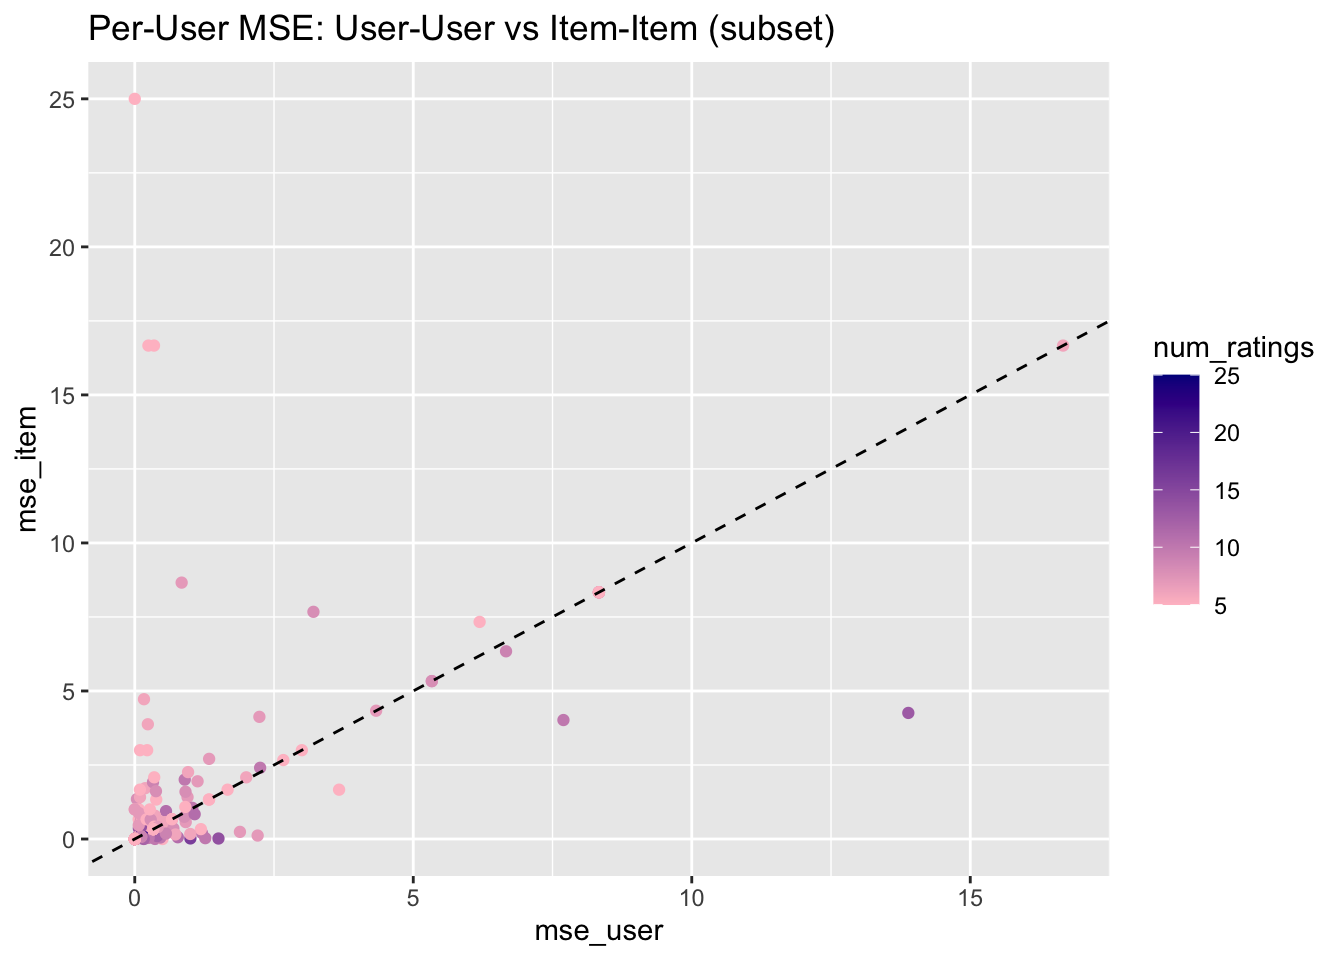
\includegraphics{CF_files/figure-latex/unnamed-chunk-10-1.pdf}

\begin{Shaded}
\begin{Highlighting}[]
\FunctionTok{ggplot}\NormalTok{(results\_df, }\FunctionTok{aes}\NormalTok{(}\AttributeTok{x =}\NormalTok{ error\_item)) }\SpecialCharTok{+} 
  \FunctionTok{geom\_histogram}\NormalTok{(}\AttributeTok{binwidth =} \FloatTok{0.5}\NormalTok{) }\SpecialCharTok{+} 
  \FunctionTok{ggtitle}\NormalTok{(}\StringTok{"Item{-}Item Prediction Error Distribution"}\NormalTok{)}
\end{Highlighting}
\end{Shaded}

\includegraphics{CF_files/figure-latex/unnamed-chunk-10-2.pdf}

\begin{Shaded}
\begin{Highlighting}[]
\CommentTok{\# which model performs better PER USER}
\NormalTok{user\_level\_perf }\OtherTok{\textless{}{-}}\NormalTok{ results\_df }\SpecialCharTok{\%\textgreater{}\%}
  \FunctionTok{group\_by}\NormalTok{(user\_id) }\SpecialCharTok{\%\textgreater{}\%}
  \FunctionTok{summarise}\NormalTok{(}
    \AttributeTok{rmse\_user =} \FunctionTok{sqrt}\NormalTok{(}\FunctionTok{mean}\NormalTok{((user\_pred }\SpecialCharTok{{-}}\NormalTok{ actual)}\SpecialCharTok{\^{}}\DecValTok{2}\NormalTok{, }\AttributeTok{na.rm =} \ConstantTok{TRUE}\NormalTok{)),}
    \AttributeTok{rmse\_item =} \FunctionTok{sqrt}\NormalTok{(}\FunctionTok{mean}\NormalTok{((item\_pred }\SpecialCharTok{{-}}\NormalTok{ actual)}\SpecialCharTok{\^{}}\DecValTok{2}\NormalTok{, }\AttributeTok{na.rm =} \ConstantTok{TRUE}\NormalTok{)),}
    \AttributeTok{mae\_user =} \FunctionTok{mean}\NormalTok{(}\FunctionTok{abs}\NormalTok{(user\_pred }\SpecialCharTok{{-}}\NormalTok{ actual), }\AttributeTok{na.rm =} \ConstantTok{TRUE}\NormalTok{),}
    \AttributeTok{mae\_item =} \FunctionTok{mean}\NormalTok{(}\FunctionTok{abs}\NormalTok{(item\_pred }\SpecialCharTok{{-}}\NormalTok{ actual), }\AttributeTok{na.rm =} \ConstantTok{TRUE}\NormalTok{)}
\NormalTok{  )}

\FunctionTok{ggplot}\NormalTok{(user\_level\_perf, }\FunctionTok{aes}\NormalTok{(}\AttributeTok{x =}\NormalTok{ rmse\_user, }\AttributeTok{y =}\NormalTok{ rmse\_item)) }\SpecialCharTok{+}
  \FunctionTok{geom\_point}\NormalTok{() }\SpecialCharTok{+}
  \FunctionTok{geom\_abline}\NormalTok{(}\AttributeTok{slope =} \DecValTok{1}\NormalTok{, }\AttributeTok{intercept =} \DecValTok{0}\NormalTok{, }\AttributeTok{linetype =} \StringTok{"dashed"}\NormalTok{) }\SpecialCharTok{+}
  \FunctionTok{labs}\NormalTok{(}\AttributeTok{title =} \StringTok{"Per{-}User RMSE: User{-}User vs Item{-}Item"}\NormalTok{)}
\end{Highlighting}
\end{Shaded}

\includegraphics{CF_files/figure-latex/unnamed-chunk-10-3.pdf}

\begin{Shaded}
\begin{Highlighting}[]
\CommentTok{\# \% of users where user{-}user is better}
\FunctionTok{mean}\NormalTok{(user\_level\_perf}\SpecialCharTok{$}\NormalTok{rmse\_user }\SpecialCharTok{\textless{}}\NormalTok{ user\_level\_perf}\SpecialCharTok{$}\NormalTok{rmse\_item)  }
\end{Highlighting}
\end{Shaded}

\begin{verbatim}
## [1] 0.4529915
\end{verbatim}

\begin{Shaded}
\begin{Highlighting}[]
\CommentTok{\# \% of users where item{-}item is better}
\FunctionTok{mean}\NormalTok{(user\_level\_perf}\SpecialCharTok{$}\NormalTok{rmse\_item }\SpecialCharTok{\textless{}}\NormalTok{ user\_level\_perf}\SpecialCharTok{$}\NormalTok{rmse\_user)  }
\end{Highlighting}
\end{Shaded}

\begin{verbatim}
## [1] 0.2307692
\end{verbatim}

\begin{Shaded}
\begin{Highlighting}[]
\NormalTok{user\_level\_perf}\SpecialCharTok{$}\NormalTok{num\_ratings }\OtherTok{\textless{}{-}} \FunctionTok{rowSums}\NormalTok{(}\SpecialCharTok{!}\FunctionTok{is.na}\NormalTok{(rating\_matrix[user\_level\_perf}\SpecialCharTok{$}\NormalTok{user\_id, ]))}

\FunctionTok{ggplot}\NormalTok{(user\_level\_perf, }\FunctionTok{aes}\NormalTok{(}\AttributeTok{x =}\NormalTok{ num\_ratings, }\AttributeTok{y =}\NormalTok{ rmse\_user }\SpecialCharTok{{-}}\NormalTok{ rmse\_item)) }\SpecialCharTok{+}
  \FunctionTok{geom\_point}\NormalTok{() }\SpecialCharTok{+}
  \FunctionTok{geom\_hline}\NormalTok{(}\AttributeTok{yintercept =} \DecValTok{0}\NormalTok{, }\AttributeTok{linetype =} \StringTok{"dashed"}\NormalTok{) }\SpecialCharTok{+}
  \FunctionTok{labs}\NormalTok{(}\AttributeTok{title =} \StringTok{"Which CF Model Performs Better by User Rating Count"}\NormalTok{,}
       \AttributeTok{y =} \StringTok{"RMSE Difference (User {-} Item)"}\NormalTok{, }\AttributeTok{x =} \StringTok{"\# of Ratings"}\NormalTok{)}
\end{Highlighting}
\end{Shaded}

\includegraphics{CF_files/figure-latex/unnamed-chunk-10-4.pdf}

We observed that user-user CF generally performs better across users,
especially those with more rating history. However, for users with fewer
than 8--10 ratings, item-item CF occasionally outperforms user-user,
likely due to stronger item similarity coverage. A hybrid approach may
help balance performance across sparse and dense users.

\end{document}
